\documentclass[a4paper,12pt]{article}
\usepackage[utf8]{inputenc}
\usepackage[bitstream-charter]{mathdesign}
\usepackage{ragged2e}
\usepackage[spanish]{babel}%Paquete de caracteres y títulos en español
\usepackage{anysize}%Paquete que permite cambiar márgenes
\marginsize{1cm}{1cm}{2cm}{2cm}
\usepackage{amsmath}%Paquete para insertar símbolos matemáticos
\usepackage{hyperref}%Paquete para insertar referencias en el texto
\usepackage{textcomp,gensymb}
\usepackage{float}%Paquete para tratar figuras y tablas como flotantes
\usepackage{lipsum}%Paquete para insertar texto mudo
\usepackage{graphicx}
\usepackage{caption}
\usepackage{subcaption}
\usepackage{url}%Paquete para insertar URL's
\usepackage{multicol}%Paquete para crear ambientes multicolumna
\setlength\columnsep{18pt}%Especifíca separación de las columnas
\renewenvironment{abstract}%Modifica el ambientes abstract para modificar la alineación
 {\par\noindent\textbf{\abstractname}\ \ignorespaces \\}
 {\par\noindent\medskip}

\title{INFORME X}
%-----------------------------------------------------------------------------------------------------------------------------------------

\begin{document}

\begin{center}
\Large{Achieving Marine Safety using Underwater Internet of Things in Smart Ocean}
\vspace{0.4cm}

\normalsize
Muthu Palaniappan M
\vspace{0.1cm}

\textit{\small{Department of CSE }\\
\small{Shiv Nadar University Chennai}}
\medskip

\normalsize

\end{center}
%-----------------------------------------------------------------------------------------------------------------------------------------

\medskip

%-----------------------------------------------------------------------------------------------------------------------------------------
\begin{multicols}{2}
%------------------------------------------------------------------------
\section{Abstract}
Marine environment monitoring has attracted more and more attention due to the growing concern about climate change.The development of the smart ocean requires that various features of the ocean be explored and understood. The Underwater Internet of Things (UIoT), an extension of the Internet of Things (IoT) to the underwater environment, constitutes powerful technology for achieving the smart ocean. s. The UIoT is enabled by the most recent developments in autonomous underwater vehicles, smart sensors, underwater communication technologies, and underwater routing protocols. At present a five-layer system architecture for the future UIoT, which consists of a sensing, communication, networking, fusion, and application layer. Finally, we suggest the current challenges and the future UIoT research trends, in which cloud computing, fog computing, and artificial intelligence are combined.\\
\\
\textbf{keywords:}
Internet of Things, Bigdata, Wireless sensor networks, marine environment, Artificial intelligence.
%--------------------------------------------------------------------------------
\section{Introduction}
AN INCREASING number of physical objects are rapidly being connected to the Internet, realizing the idea of the Internet of Things (IoT). In recent years, the IoT has developed rapidly and enabled numerous applications with different characteristics in many fields, such as the smart home, transportation, healthcare, industrial automation, and emergency response. For human, the ocean not only has a large amount of oil, gas, and fish resources, but is also an important channel for the international trade and a potential energy resource, such as tidal energy and the kinetic energy of the ocean currents. However, there remains a lack of intelligent and convenient applications for the ocean because of the complexity of the underwater environment and the expense of the underwater equipment. As an extension of the IoT in the underwater environment, the Underwater IoT is increasingly becoming a powerful technology for developing the smart ocean. Here, Underwater IoT is defined as UIoT that is a smart network with self-learning and intelligent computing capabilities. It can sense, monitor, and identify underwater objects by wired or wireless communication for building smart ocean.\\

Although the unique characteristics of the ocean can bestow many benefits on humans, they also restrict the development of the UIoT. Hence, the model and design of the land-based IoT cannot be adopted directly by the UIoT. For instance, ocean currents constitute a nonnegligible issue for the deployment of the UIoT . Underwater node movement in the UIoT caused by ocean currents often affects network coverage and data transmission quality. Moreover, the mode of the underwater acoustic communication (UAC) seriously restricts the efficiency of data transmission because of the UAC characteristics such as high cost, narrow bandwidth, high bit error rate, slow transmission speed, and high energy consumption. In addition, the battery power of UIoT sensor nodes is severely limited, and node batteries cannot be conveniently recharged owing to the limitation of seawater corrosion and seawater pressure. Therefore, the future UIoT should connect underwater entities intelligently, as does the existing Internet of Underwater Things. More importantly, artificial intelligence and fog computing need to be combined to provide the UIoT network with certain self-learning and intelligent computing capabilities so that it can be adapted to the complex underwater environment and meet the different needs of marine applications. \\

An UIoT model, shown in Fig. 1, usually includes underwater sensing and transmission modules (underwater sensor nodes and surface nodes), underwater computing and transmission modules [autonomous underwater vehicles (AUVs)], surface computing and transmission modules [surface base station (BS), surface ships, and surface nodes], and coastal control modules (seashore BS and seashore control center). A simple operating process of the UIoT is described later. A large number of valuable ocean data are collected by underwater sensor nodes at first. Then, the data are completed corresponding data fusion and intelligent computing when transmitted by underwater nodes and AUVs. Underwater nodes and AUVs use a variety of underwater communication technologies to transmit data to surface computing and transmission modules. Some underwater valuable data are analyzed by edge servers on surface in surface for the underwater network and marine applications (exploration platform and deep range, etc.), and the rest are transmitted to Internet cloud servers or seashore control centers via radio communications. Seashore control centers generate a series of intelligent decisions based on the data collected from the ocean and Internet cloud servers to facilitate human activities in the ocean. Furthermore, underwater wireless sensor networks (UWSNs), which can provide ocean information and improve users ability to monitor and forecast events in the underwater environments, are also an important part of the UIoT.\\

\section{UIoT system Architecture}
The UIoT is a complex system comprising multiple heterogeneous networks; hence, a flexible layered system architecture is critically needed. Many different IoT system architectures based on the analysis of the needs of researchers and industry exist. However, few UIoT system architectures have been proposed. A basic system architecture of the UIoT was proposed, which has three layers: the application layer, network layer, and perception layer. In this article, we propose a five-layer UIoT system architecture, which consists of two parts, underwater and non underwater, as shown in Fig. 2. The UIoT system architecture includes an application, fusion, networking, communication, and sensing layer. Each layer of the system architecture has an independent function and scalability. In addition, we will discuss the application of cloud computing, fog computing, and artificial intelligence in this UIoT system architecture. These technologies have great impact on the development of the IoT. For cloud computing in it is defined as a model for enabling ubiquitous, convenient, on-demand network access to a shared pool of configurable computing resources that can be rapidly provisioned and released with minimal management effort or service provider interaction. As an extension of cloud computing, fog computing is more time sensitive, which is a highly virtualized platform that provides compute, storage, and networking services between end devices and traditional cloud server. Machine learning algorithms in artificial intelligence can solve several challenges of the UIoT, such as objects targeting, event detection, data transmission, network security, and quality of service. Machine learning is described as the adoption of computational methods for improving the machine performance by detecting and describing consistencies and patterns in training data. In the following, we describe the five layers of our proposed UIoT system architecture.\\
\\
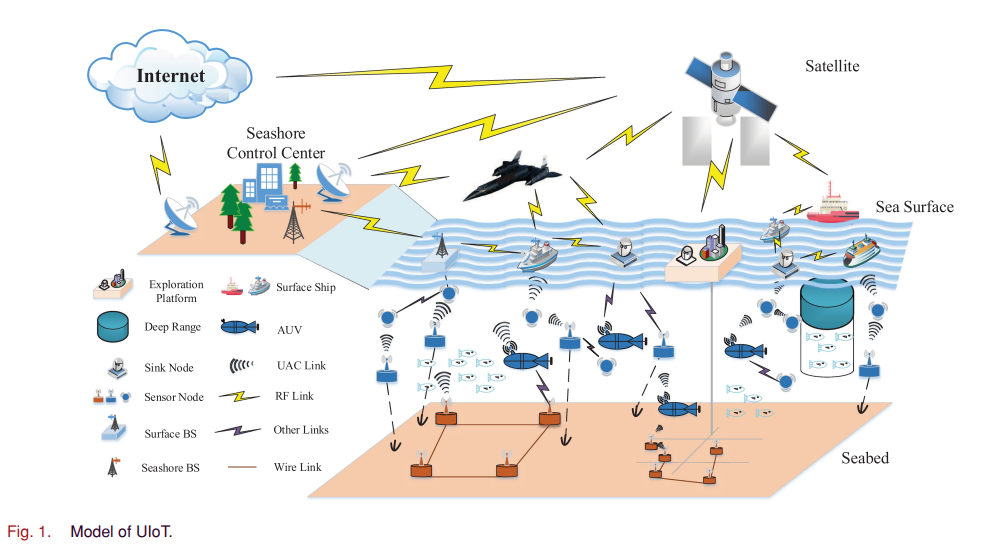
\includegraphics[width=8cm,height=10cm,keepaspectratio]{fig1.png}
\section{Layers of architecture}

\item\textbf{Sensing layer}\\
\\
In the sensing layer, the various sensors, such as temperature, flow velocity, salinity, and motion sensors, and cameras provide meaningful sensing data and identification data for various underwater applications to supply records and assist in decision making. Compared with sensor nodes of the IoT, underwater sensor nodes of the UIoT need to have the ability of self-target recognition for initially validating the value of the data in complex and changeable underwater environment. For example, a turbid underwater environment can cause many worthless image data to be generated. It is needed to reduce energy consumption of worthless data transmission because the cost of transmitting data in underwater is huge and underwater sensor nodes are often given more computing power. The underwater self-target recognition of underwater sensor nodes can be realized by many machine learning algorithms, such as neural network, support vector machine, deep learning, etc. In the UIoT, the sensors are deployed in monitoring areas, and a self-organizing topology, which is required by the dynamic underwater environment, is constructed. A typical UWSN system includes underwater sensor nodes, surface sink nodes, and surface management nodes. The sensing data from underwater sensor nodes are transmitted to surface sink nodes by multihop links quickly and reliably. Then, the sink node processes or transmits the data to the monitoring center. Users manage the sensor network and issue monitoring task commands through the surface management nodes. Furthermore, underwater sensor nodes are expensive at present, so their maintenance and upgrading need further attention with the increasing worldwide attention given to the ocean.

\item\textbf{Communication Layer}\\
\\
The main function of the UIoT communication layer is to allocate the corresponding underwater communication technology to be used for data transmission based on business requirements, task categories, and data importance. Because radio communication, which is usually used in the IoT, cannot be adapted to the underwater environment, the underwater part of the UIoT has many other communication modes with different levels of performance, such as UAC, optical wireless communication, and magnetic induction communication. However, on the comprehensive performance of transmission efficiency and reliability, any single underwater wireless communication technology cannot be compared with that of radio communication. The communication distance of the UAC is long, but its bandwidth is narrow in contrast to that of wireless optical communication. In the underwater environment, the transmission stability of the magnetic induction communication is better than that of the wireless optical communication and UAC. In addition, the communication rate of the UAC is proportional to the frequency, whereas the communication distance is inversely proportional to the frequency. Therefore, in order to further promote the development of the UIoT, these underwater communication technologies need be combined to form many underwater multimodal communication systems (UMCSs) with different characteristics for various UIoT applications. An UMCS is defined as the system encompasses any set of non-mutually interfering underwater communication technologies, which may have various advantages from different communication technologies. For an UMCS, it can be designed by including UAC and underwater optical communication (UOC). It even can be built by a set of UAC modules working on different bands. Because they have some complementary features such as low-frequency acoustic communications achieve kbit/s transmission rates over ranges of a few kilometers, and high-frequency acoustics tops tens of kbit/s over up to a few hundred meters.
\\

\item\textbf{Networking Layer}\\
\\
In the UIoT, the networking layer is used to construct an efficient topology for transferring the data produced by the sensing layer to the fusion layer through underwater multimodal channels and radio communication above the water. The UIoT network model of above water part is similar to that of the IoT. Here, we focus on the underwater network part of the networking layer of the UIoT. The underwater network model of the UIoT needs to be presented that provide an efficient and reliable data transmission capacity for nodes, because of the poor communication channels, unfixed node location, and limited energy supply. In the underwater network part, underwater vehicles and AUVs, as two super nodes of the underwater network, can significantly improve the underwater network performance, in terms of robustness and connectivity. Meanwhile, in order to improve the efficiency of data transmission in underwater, the UMCS networking strategies using a variety of underwater communication technologies and underwater nodes are becoming a research hotspot. However, the demand for ocean big data transmission in underwater is still not fully met. Therefore, the future UIoT will need a high data transmission capacity to forward the big data to fusion layer. Machine learning is widely used in many fields because of its excellent analytical ability. It is a potential tool to further improve network performance because a variety of machine learning methods can learn network state and environment parameters adaptively, such as reinforcement learning, broad learning, deep learning , decision tree, and self-organizing map. Hence, a self-learning and self-organizing routing algorithm based on learning the changes in the underwater environment should be adopted to further optimize the underwater network model of the UIoT.
\\

\item\textbf{Application Layer}\\
\\
The application layer of the UIoT uses the ocean data processed by the fusion layer to provide convenient and intelligent services to users according to their requirements. Various intelligent functions based on machine learning are adopted to enable application managers to better address user needs and to improve user comfort in using the UIoT applications, for example, smart language recognition, smart image recognition, and smart preference recommendation, etc. These machine learning techniques includes hidden Markov model, discriminative learning, structured sequence learning, Bayesian learning, and deep learning. Moreover, an important responsibility of the application layer is to protect user privacy security. The cloud servers can remotely control underwater intelligent nodes and robots based on the analytical data results. Currently, the main applications of the UIoT are as follows: environmental monitoring, resource exploration, disaster preparations, military application, sea rescue, and offshore entertainment. The categories of the existing UIoT applications are shown in Table I. In addition, with the development of the smart ocean, potential applications of the UIoT exist that should be seriously considered, such as smart monitoring of fish stocks and feeding environments in the deep range (the deep range monitoring network) and a design system for seabed tourist routes (underwater tourism network). UIoT applications are utilized daily to make maritime activities safer and more convenient.
\\
\\
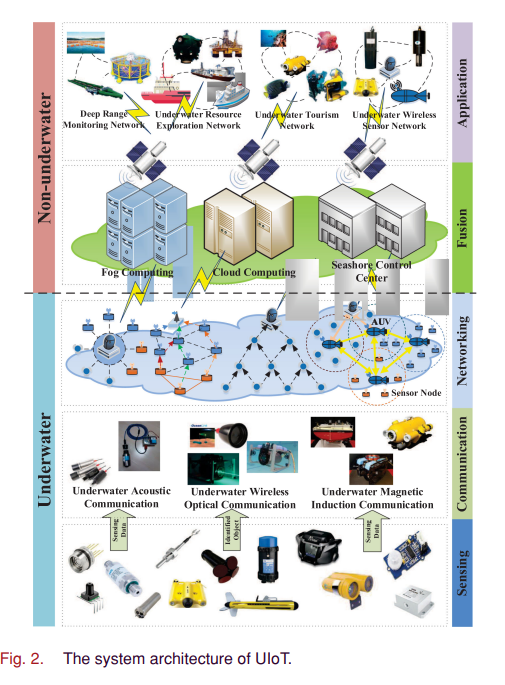
\includegraphics[width=8cm,height=10cm,keepaspectratio]{fig2.png}
\section{Protocols}
Working of underwater networking strategy.
\\
\item \textbf{A)	Node Mobility and Equipment Heterogeneity Impairs the Reliability of Underwater Networking}\\
\\
The mobility of the ocean current is a unavoidable issue in the networking of underwater sensors in the UIoT. An interruption of the underwater network of the UIoT is easily incurred, and therefore, the reliability of the network topology is seriously challenged. In addition, the accuracy of the underwater localization is also affected mainly by the movement of currents. Although there are some ocean current models that have been applied in UIoT simulations, these models cannot accurately represent the actual ocean environment, because the ocean current is affected by many factors, such as wind and temperature. This greatly increases the difficulty of underwater networking. Meanwhile, the UIoT is a complex system that consists of many heterogeneous network elements. The underwater network part of the UIoT includes underwater acoustic networks, underwater wireless optical communication networks, underwater magnetic induction networks, and the dynamic wireless network based on AUVs. The features of these heterogeneous network elements vary widely, and the heterogeneity of devices, technologies, and services presents many serious challenges. The optimization of all the network elements of the UIoT can be coordinated for communication, and the maximization of the efficiency of each underwater network is also an important future challenge for researchers.\\

\item\textbf{B)	Exploration of Highly Reliable and Self-Adaptive Networking Strategy for Large-Scale Perception of the UIoT:}\\
\\
In the UIoT, a large number of distributed underwater sensing nodes that form the underwater network part are integrated through self-organizing routing protocols [97] and topology control strategies. These nodes collaborate on data communication to ensure that data can be sent to the sink node or the control center. Because of the complex underwater environment and inefficient and unreliable underwater communication technology, the reliability of underwater networks is poor. In particular, when the scale of the underwater network is large, the existing networking strategies are not suitable. Machine learning-based networking and routing strategies for large-scale terrestrial wireless sensor networks in IoT have been extensively studied, because of its strong adaptive and computational capabilities. Various underwater network performance of the UIoT is difficult to control and optimize by the traditional methods that are used for the IoT because the marine environment is more complex and changeable than the terrestrial environment.

\section{Realization of the Smart Ocean}\\
The smart ocean is widely applied in ocean activities closely related to humans, such as smart ocean pollution monitoring, smart deep range monitoring, smart underwater navigation, smart underwater resource exploration, smart underwater tourism, smart disaster warning, and smart underwater intrusion detection. It can help people understand the ocean more comprehensively, utilize the ocean’s potentials more fully, and govern the ocean more conveniently so that it serves humankind better. The smart ocean requires that the UIoT transmit, calculate, process, and protect various valuable data in the ocean. That is, the realization of the smart ocean depends on the above five research points of the UIoT: underwater wireless communication, underwater networking, cooperative computing, security, and standardization. The acceleration of the research of these aspects for the UIoT is of great significance to the development of smart oceans.\\

\section{Conclusion}
The future UIoT will be based on oceanography, underwater sensor technology, underwater multimodal communication technology, hybrid networks, cooperative computing, fog computing, and cloud computing to construct the smart ocean. In this article, we examined the existing survey papers on the UIoT and presented our proposed five-layer UIoT system architecture, where the sensing layer focuses on monitoring sensing data from smart sensor devices in the ocean. We discussed the typical features of the underwater communication in the communication layer. For the networking layer, the routing strategy for underwater part of the UIoT was discussed. In the fusion layer, the different approaches for decision making based on cloud computing and fog computing were examined. Then, we classified the existing typical applications of the UIoT and proposed some potential applications for the application layer. Finally, we highlighted the issues and challenges of the UIoT that must be addressed in the future to build smart oceans,and envisioned the open issues in the UIoT research. We hope that this article will facilitate researchers and developers being able to understand the perspectives and challenges of developing the UIoT.


%--------------------------------------------------------------------------------------------------
\end{multicols}
%----------------------------------------------------------------------------------


\end{document}